
\documentclass[8pt]{beamer}

\usepackage[T1]{fontenc}
\usepackage{lmodern} % must be loaded with fontenc --- otherwise text will become bitmaps
\usepackage[british]{babel}
\usepackage{csquotes} % will automatically use quotes of the babel language
\usepackage{amssymb}
\usepackage{amsmath}
\usepackage{amsthm}
\usepackage{microtype}
\usepackage{mathtools}
\usepackage{etoolbox}
\usepackage{tabularx}
\usepackage{booktabs}
\usepackage{listings}
\usepackage{color}
\usepackage[normalem]{ulem}
\usepackage[style=apa]{biblatex} % verbose or apa depending on cite style
\usepackage{xcolor}
\usepackage[capitalize]{cleveref} % use capitalization so that we do not need to worry about detecting beginnings of sentences, etc
\usepackage{import}
\usepackage[useregional]{datetime2}
\usepackage{physics}
\usepackage{float} % for H option in table
\usepackage{parskip} % remove indentation on new paragraphs
\usepackage{caption}
\usepackage[export]{adjustbox} % allow max width
\usepackage{graphbox} % allow align=t in \includegraphics to make them work better in minipages if first item
\usepackage{appendixnumberbeamer}

\MakeOuterQuote{"}

\lstset{
	backgroundcolor=\color[rgb]{1,1,1},
	tabsize=4,
	rulecolor=,
	basicstyle=\ttfamily,
	upquote=true,
	aboveskip={1.5\baselineskip},
	columns=fixed,
	showstringspaces=false,
	extendedchars=true,
	breaklines=true,
	prebreak = \raisebox{0ex}[0ex][0ex]{\ensuremath{\hookleftarrow}},
	showtabs=false,
	showspaces=false,
	showstringspaces=false,
	identifierstyle=\ttfamily,
	keywordstyle=\color[rgb]{0,0,1},
	commentstyle=\color[rgb]{0.133,0.545,0.133},
	stringstyle=\color[rgb]{0.627,0.126,0.941},
	aboveskip=0pt,
	literate={£}{{\textsterling{}}}1 % allow £ sign within listings
}

\newcommand{\noncolouredtableofcontents}{
	\begingroup
	\hypersetup{hidelinks}
	\tableofcontents
	\endgroup
}

\ifcsundef{thematicbreak}{\newcommand{\thematicbreak}{\par\bigskip\noindent\hrulefill\par\bigskip}}{}

\theoremstyle{definition}
\ifcsundef{definition}{\newtheorem{definition}{Definition}[section]}{}

\theoremstyle{plain}
\ifcsundef{theorem}{\newtheorem{theorem}{Theorem}[section]}{}
\ifcsundef{lemma}{\newtheorem{lemma}[theorem]{Lemma}}{}
\ifcsundef{corollary}{\newtheorem{corollary}{Corollary}[theorem]}{}

\theoremstyle{definition}
\ifcsundef{definition}{\newtheorem{definition}{Definition}[section]}{}
\ifcsundef{example}{\newtheorem{example}{Example}[section]}{}

\theoremstyle{remark}
\ifcsundef{assumption}{\newtheorem*{assumption}{Assumption}}{}
\ifcsundef{proof}{\newtheorem*{proof}{Proof}}{}
\ifcsundef{exercise}{\newtheorem{exercise}{Exercise}[section]}{}
\ifcsundef{problem}{\newtheorem{problem}{Problem}[section]}{}
\ifcsundef{question}{\newtheorem{question}{Question}[section]}{}
\ifcsundef{tip}{\newtheorem*{tip}{Tip}}{}
\ifcsundef{solution}{\newtheorem*{solution}{Solution}}{}
\ifcsundef{note}{\newtheorem{note}{Note}[section]}{}
\ifcsundef{derivation}{\newtheorem{derivation}{Derivation}[section]}{}
\ifcsundef{axiom}{\newtheorem{axiom}{Axiom}[section]}{}
\ifcsundef{conjecture}{\newtheorem{conjecture}{Conjecture}[section]}{}
\ifcsundef{hypothesis}{\newtheorem{hypothesis}{Hypothesis}[section]}{}
\ifcsundef{proposition}{\newtheorem{proposition}{Proposition}[section]}{}

\ifcsundef{remark}{\newtheorem*{remark}{Remark}}{} % notes are numbered but remarks are not

\renewcommand{\qedsymbol}{$\blacksquare$} % closed black square for proof environments

\renewcommand\thesection{\arabic{section}}

\numberwithin{equation}{section}
\numberwithin{figure}{section}
\numberwithin{table}{section}

\providecommand{\tightlist}{%
  \setlength{\itemsep}{0pt}\setlength{\parskip}{0pt}}
  
% fix parskip within minipage
\setlength{\parskip}{\medskipamount}
\makeatletter
\newcommand{\@minipagerestore}{\setlength{\parskip}{\medskipamount}}
\newcommand{\mathcolorbox}[2]{\colorbox{#1}{$\displaystyle #2$}}
\makeatother

\newcommand*{\matr}[1]{\mathbfit{#1}}
\newcommand*{\tran}{^{\mkern-1.5mu\mathsf{T}}}
\newcommand*{\conj}[1]{\overline{#1}}
\newcommand*{\hermconj}{^{\mathsf{H}}}

\usepackage{tikz}
\usepackage[tikz]{ocgx2}
\usetikzlibrary{tikzmark, fit, calc, positioning,arrows.meta}

\bibliography{bib.bib}


\usetheme{Rochester}
\usefonttheme{structureitalicserif}



% \usefonttheme{serif}

% remove indent from itemize
\settowidth{\leftmargini}{\usebeamertemplate{itemize item}}
\addtolength{\leftmargini}{\labelsep}

\setbeamersize{text margin left=2em,text margin right=2em} 

\setbeamerfont{institute}{size=\normalsize}

% \setbeamerfont{title}{series=\bfseries,parent=structure}
% \setbeamerfont{frametitle}{series=\bfseries,parent=structure}

\date[15/01/24]{15th January 2024}
\title[Discontinuous Constituent Parsing]{Multitask Pointer Network for Discontinuous Constituent Parsing}
\subtitle[An application to German]{An application to the German language}
\author[J. Yu]{James Yu \newline \href{mailto:jby21@cam.ac.uk}{\texttt{jby21@cam.ac.uk}}}
\institute[Cambridge]{Faculty of Economics \\ University of Cambridge}


\begin{document}

\begin{frame}
    \titlepage
\end{frame}

\section{Introduction}
\subsection{Motivation}
\begin{frame}
    \frametitle{Why use a neural network to model grammar?}
\end{frame}

\subsection{Preliminaries}
\begin{frame}
    \frametitle{Linguistic preliminaries: constituent trees}
    Let \(w = \qty(w_{1}, \ldots, w_{L})\) be a sentence.

    \begin{definition}
        \begin{itemize}
            \item A \textit{constituent tree} is a rooted tree whose leaves are the words \(\qty(w_{i})_{i=1}^{L}\) and internal nodes are constituents satisfying some constraints.

            \item A \textit{constituent} is a triple \(\qty(\tikzmarknode{const-label}{Z}, \tikzmarknode{const-yield}{\mathcal{Y}}, \tikzmarknode{const-head}{h})\) containing, respectively, its label, yield, and lexical head.
            
            \item A constituent is \tikzmarknode{disc-text}{\textit{discontinuous}} if its yield is not contiguous.
        \end{itemize}
    \end{definition}

    \begin{figure}
        \centering
        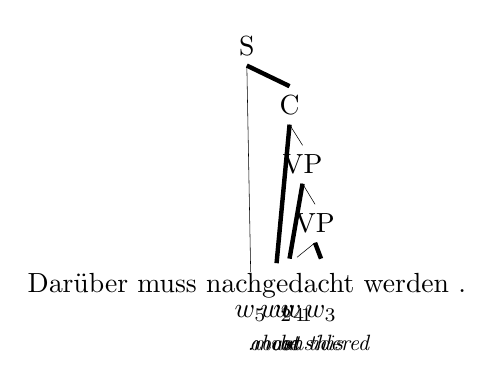
\begin{tikzpicture}[remember picture]
            \node[inner sep=0, text depth=0] (w) {\subnode[inner sep=0]{s-yld}{\subnode[inner sep=0]{c-yld}{\subnode[inner sep=0]{vptop-left}{\subnode[inner sep=0]{vpbot-left}{\subnode[inner sep=2pt]{w1}{Darüber}}} \subnode[inner sep=2.5pt]{w2}{muss} \subnode[inner sep=0]{vptop-right}{\subnode[inner sep=0]{vpbot-right}{\subnode[inner sep=1.5pt]{w3}{nachgedacht}} \subnode[inner sep=1.5pt]{w4}{werden}}} \subnode[inner sep=2.5pt]{w5}{.}}};
        
            \foreach \n/\english in {1/about this,2/must,3/considered,4/be,5/.} \node[below=1ex of {w\n |- w.south}, inner sep=0, align=center] {\(w_{\n}\) \\[0ex] \scalebox{0.8}{\textit{\english}}};
            
            % \coordinate (s) at ({barycentric cs:w1=1,w2=1,w3=1,w4=1} |- {barycentric cs:w=1,vroot=4});
            
            \node[switch ocg=const-s] (vroot) at ($(w) + (0, 3cm)$)  {S};
            \node[switch ocg=const-c] (s) at ({barycentric cs:w1=1,w2=3,w3=1,w4=1} |- {barycentric cs:w=1,vroot=3}) {C};
            \node[switch ocg=const-vptop] (vp1) at ({barycentric cs:w1=1,w3=1,w4=1} |- {barycentric cs:w=2,vroot=2}) {VP};
            \node[switch ocg=const-vpbot] (vp2) at ({barycentric cs:w1=1,w3=3} |- {barycentric cs:w=3,vroot=1}) {VP};
        
            \draw[very thin] (vroot.south) -- (w5.north);
            \draw[ultra thick] (vroot.south) -- (s.north);
            \draw[ultra thick] (s.south) -- (w2.north);
            \draw[very thin] (s.south) -- (vp1.north);
            \draw[ultra thick] (vp1.south) -- (w4.north);
            \draw[very thin] (vp1.south) -- (vp2.north);
            \draw[very thin] (vp2.south) -- (w1.north);
            \draw[ultra thick] (vp2.south) -- (w3.north);
        \end{tikzpicture}
    \end{figure}
    
    \begin{tikzpicture}[remember picture, overlay]
        % vptop
        \begin{scope}[ocg={ref=const-vptop, status=invisible, opts={radiobtngrp=const}}]
            \node[draw, fit=(vp1), fill=red, inner sep=0, opacity=0.5] {};
            \node[draw, fit=(vptop-right), fill=green, inner sep=0, minimum height=1em, opacity=0.5] {};
            \node[draw, fit=(vptop-left), fill=green, inner sep=0, minimum height=1em, opacity=0.5] {};
            \node[draw, fit=(w4), fill=cyan, inner sep=0, minimum height=1em, opacity=0.5] {};
            \draw[ultra thick, cyan] (vp1.south) -- (w4.north);
    
            % highlight in definition
            \node[draw, fit=(const-label), fill=red, inner sep=0, opacity=0.5] {};
            \node[draw, fit=(const-yield), fill=green, inner sep=0, opacity=0.5] {};
            \node[draw, fit=(const-head), fill=cyan, inner sep=0, opacity=0.5] {};
            \node[draw, fit=(disc-text), fill=yellow, inner sep=0, opacity=0.5] {};
        \end{scope}
    
        % vpbot
        \begin{scope}[ocg={ref=const-vpbot, status=invisible, opts={radiobtngrp=const}}]
            \node[draw, fit=(vp2), fill=red, inner sep=0, opacity=0.5] {};
            \node[draw, fit=(vpbot-right), fill=green, inner sep=0, minimum height=1em, opacity=0.5] {};
            \node[draw, fit=(vpbot-left), fill=green, inner sep=0, minimum height=1em, opacity=0.5] {};
            \node[draw, fit=(w3), fill=cyan, inner sep=0, minimum height=1em, opacity=0.5] {};
            \draw[ultra thick, cyan] (vp2.south) -- (w3.north);
    
            % highlight in definition
            \node[draw, fit=(const-label), fill=red, inner sep=0, opacity=0.5] {};
            \node[draw, fit=(const-yield), fill=green, inner sep=0, opacity=0.5] {};
            \node[draw, fit=(const-head), fill=cyan, inner sep=0, opacity=0.5] {};
            \node[draw, fit=(disc-text), fill=yellow, inner sep=0, opacity=0.5] {};
        \end{scope}
    
        % c-yld
        \begin{scope}[ocg={ref=const-c, status=invisible, opts={radiobtngrp=const}}]
            \node[draw, fit=(s), fill=red, inner sep=0, opacity=0.5] {};
            \node[draw, fit=(c-yld), fill=green, inner sep=0, minimum height=1em, opacity=0.5] {};
            \node[draw, fit=(w2), fill=cyan, inner sep=0, minimum height=1em, opacity=0.5] {};
            \draw[ultra thick, cyan] (s.south) -- (w2.north);
    
            % highlight in definition
            \node[draw, fit=(const-label), fill=red, inner sep=0, opacity=0.5] {};
            \node[draw, fit=(const-yield), fill=green, inner sep=0, opacity=0.5] {};
            \node[draw, fit=(const-head), fill=cyan, inner sep=0, opacity=0.5] {};
        \end{scope}
    
        % s-yld
        \begin{scope}[ocg={ref=const-s, status=invisible, opts={radiobtngrp=const}}]
            \node[draw, fit=(vroot), fill=red, inner sep=0, opacity=0.5] {};
            \node[draw, fit=(s-yld), fill=green, inner sep=0, minimum height=1em, opacity=0.5] {};
            \node[draw, fit=(w2), fill=cyan, inner sep=0, minimum height=1em, opacity=0.5] {};
            \draw[ultra thick, cyan] (vroot.south) -- (s.north);
            \draw[ultra thick, cyan] (s.south) -- (w2.north);
            
            % highlight in definition
            \node[draw, fit=(const-label), fill=red, inner sep=0, opacity=0.5] {};
            \node[draw, fit=(const-yield), fill=green, inner sep=0, opacity=0.5] {};
            \node[draw, fit=(const-head), fill=cyan, inner sep=0, opacity=0.5] {};
        \end{scope}
    \end{tikzpicture}
\end{frame}

\begin{frame}
    \frametitle{Reduction to dependency parsing}

    \begin{definition}
        A \textit{dependency tree} is a rooted tree spanning the words in the sentence \(\qty(w_{i})_{i=1}^{L}\). Each edge is labelled and connects a \textit{head word} (parent) to a \textit{dependency} (child).
    \end{definition}

    \textcite{fernandez2015parsing} show that constituent trees are isomorphic to dependency trees in which the edges contain information about constituent labels and attachment order.

    \begin{columns}[onlytextwidth]
        \begin{column}{0.45\textwidth}
            \begin{figure}
                \centering
                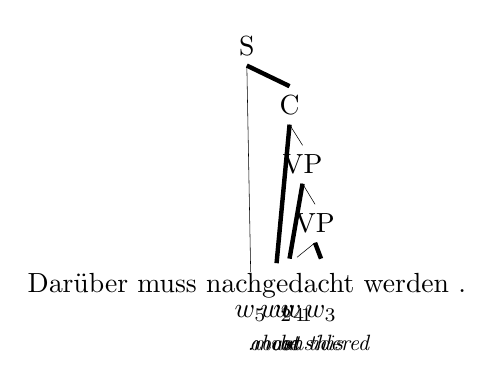
\begin{tikzpicture}[remember picture]
                    \node[inner sep=0, text depth=0] (wc) {\subnode[inner sep=0]{sc-yld}{\subnode[inner sep=0]{cc-yld}{\subnode[inner sep=0]{vptopc-left}{\subnode[inner sep=0]{vpbotc-left}{\subnode[inner sep=2pt]{wc1}{Darüber}}} \subnode[inner sep=2.5pt]{wc2}{muss} \subnode[inner sep=0]{vptopc-right}{\subnode[inner sep=0]{vpbotc-right}{\subnode[inner sep=1.5pt]{wc3}{nachgedacht}} \subnode[inner sep=1.5pt]{wc4}{werden}}} \subnode[inner sep=2.5pt]{wc5}{.}}};
                
                    \foreach \n/\english in {1/about this,2/must,3/considered,4/be,5/.} \node[below=1ex of {wc\n |- wc.south}, inner sep=0, align=center] {\(w_{\n}\) \\[0ex] \scalebox{0.8}{\textit{\english}}};
                    
                    % \coordinate (s) at ({barycentric cs:w1=1,w2=1,w3=1,w4=1} |- {barycentric cs:w=1,vroot=4});
                    
                    \node[switch ocg=constc-s] (vrootc) at ($(wc) + (0, 3cm)$)  {S};
                    \node[switch ocg=constc-c] (sc) at ({barycentric cs:wc1=1,wc2=3,wc3=1,wc4=1} |- {barycentric cs:wc=1,vrootc=3}) {C};
                    \node[switch ocg=constc-vptop] (vpc1) at ({barycentric cs:wc1=1,wc3=1,wc4=1} |- {barycentric cs:wc=2,vrootc=2}) {VP};
                    \node[switch ocg=constc-vpbot] (vpc2) at ({barycentric cs:wc1=1,wc3=3} |- {barycentric cs:wc=3,vrootc=1}) {VP};
                
                    \draw[very thin] (vrootc.south) -- (wc5.north);
                    \draw[ultra thick] (vrootc.south) -- (sc.north);
                    \draw[ultra thick] (sc.south) -- (wc2.north);
                    \draw[very thin] (sc.south) -- (vpc1.north);
                    \draw[ultra thick] (vpc1.south) -- (wc4.north);
                    \draw[very thin] (vpc1.south) -- (vpc2.north);
                    \draw[very thin] (vpc2.south) -- (wc1.north);
                    \draw[ultra thick] (vpc2.south) -- (wc3.north);
                \end{tikzpicture}
            \end{figure}
        \end{column}
        \begin{column}{0.1\textwidth}
            \tikz\draw[blue,thick,Stealth-Stealth] (0,0) -- (\textwidth,0);
        \end{column}
        \begin{column}{0.45\textwidth}
            \begin{figure}
                \centering
                
\begin{tikzpicture}[remember picture]
                    \node[inner sep=0, text depth=0] (w) at (0,0) {\subnode[inner sep=2pt]{wd1}{Darüber} \subnode[inner sep=2.5pt]{wd2}{muss} \subnode[inner sep=1.5pt]{wd3}{nachgedacht} \subnode[inner sep=1.5pt]{wd4}{werden} \subnode[inner sep=2.5pt]{wd5}{.}};
            
                    % muss
                    \draw[-Stealth] ($(wd2.north) + (2pt, 0)$) to [bend left=50] node [above, scale=0.5] {C\#1} ($(wd4.north) + (2pt, 0)$);
                    \draw[-Stealth] ($(wd2.north) + (2pt, 0)$) to [bend left=80] node [above, scale=0.5] (s2) {S\#2} (wd5.north);
            
                    % werden
                    \draw[-Stealth] ($(wd4.north) - (2pt, 0)$) to [bend right=30] node [above, scale=0.5] {VP\#1} ($(wd3.north) + (2pt, 0)$);
            
                    % nachgedacht
                    \draw[-Stealth] ($(wd3.north) - (2pt, 0)$) to [bend right=60] node [above, scale=0.5] {VP\#1} (wd1.north);
            
                    % % root
                    % \node[scale=0.5] (root) at ({$(wd2) - (2pt, 0)$} |- s2) {\texttt{root}};
                    % \draw[-Stealth] (root.south) -- (root |- wd2.north);

                    \foreach \n in {1,2,3,4,5} \node[below=1ex of {wd\n |- w.south}, inner sep=0, align=center] {\(w_{\n}\)};
                \end{tikzpicture}
            \end{figure}
        \end{column}
    \end{columns}
\end{frame}

\section{Model}
\subsection{Mathematical Formulation}
\begin{frame}
    \frametitle{Mathematical formalisation}
    \begin{columns}[t,onlytextwidth]
        \begin{column}[t]{0.6\textwidth}
            \vspace{0pt}
            \begin{itemize}
                \item Regressor: sentence \(\qty(w_{i})_{i = 1}^{L}\).
                \item Regressand: dependency tree, parts of speech and morphology.
                \item Bottom-up approach: think of \textit{arcs} going from every child \(w_{i}\) to its parent \(y_{i}^{\text{arc}} \in w \setminus w_{i}\).
            \end{itemize}
        \end{column}
        \begin{column}[t]{0.4\textwidth}
            % \begin{figure}
                \raggedleft
                \scalebox{0.8}{
\begin{tikzpicture}[remember picture,baseline=(current bounding box.north west)]
                    \node[font=\small,inner sep=0, text depth=0] (wdd) at (0,0) {\subnode[inner sep=0]{start}{\hspace{3em}} \subnode[inner sep=2pt]{wdd1}{Darüber} \subnode[inner sep=2.5pt]{wdd2}{muss} \subnode[inner sep=1.5pt]{wdd3}{nachgedacht} \subnode[inner sep=1.5pt]{wdd4}{werden} \subnode[inner sep=2.5pt]{wdd5}{.}};
            
                    % lines and text
                    % muss
                    \draw[blue,thick,Stealth-] ($(wdd2.north) + (6pt, 0)$) to [bend left=50] node [black,above, scale=0.5] {C\#1} ($(wdd4.north) + (2pt, 0)$);
                    \draw[blue,thick,Stealth-] ($(wdd2.north) + (3pt, 0)$) to [bend left=80] node [black,above, scale=0.5] (s2) {S\#2} (wdd5.north);
            
                    % werden
                    \draw[blue,thick,Stealth-] ($(wdd4.north) - (2pt, 0)$) to [bend right=30] node [black,above, scale=0.5] {VP\#1} ($(wdd3.north) + (2pt, 0)$);
            
                    % nachgedacht
                    \draw[blue,thick,Stealth-] ($(wdd3.north) - (2pt, 0)$) to [bend right=60] node [black,above, pos=0.45, scale=0.5] {VP\#1} (wdd1.north);
            
                    % root
                    \node[black,scale=0.5] (root) at ({$(wdd2) - (2pt, 0)$} |- s2) {\texttt{(root)}};
                    \draw[blue,thick,Stealth-] (root.south) -- (root |- wdd2.north);

                    % word number labels
                    \foreach \n in {1,2,3,4,5} \node[below=1ex of {wdd\n |- wdd.south}, inner sep=0, align=center] (wddlab\n) {\(w_{\n}\)};

                    % regressand labels
                    \foreach \i/\m in {1/{0/\(w_{3}\),1/VP,2/1,3/PAV,4/--},2/{0/\texttt{(root)},1/--,2/--,3/VM,4/fin},3/{0/\(w_{4}\),1/VP,2/1,3/V,4/part},4/{0/\(w_{2}\),1/C,2/1,3/VA,4/inf},5/{0/\(w_{2}\),1/S,2/2,3/\$.,4/--}}
                    {
                        \foreach \j/\k in \m
                        {
                            \node[scale=0.8,gray,inner sep=0] (pos\i\j) at ($({wdd\i.center |- wddlab1.south}) - (0, 4pt) - (0, 1.7ex * \j) $) {\k};
                        }
                    }
            
                    \node[inner sep=0,anchor=west] at (start.west |- wdd1) {\(w\)};
                    \foreach \j/\t in {0/arc,1/lab,2/ord,3/pos,4/morph}
                    {
                        \node[scale=0.8,gray,inner sep=0,anchor=west] at (start.west |- pos2\j) {\(y^{\text{\t}}\)};
                    }
                \end{tikzpicture}}
            % \end{figure}        
        \end{column}
    \end{columns}

    Denote the regressand by \(y = \qty(y_{i})_{i=1}^{L}\) where \(y_{i} = (y_{i}^{\text{arc}}, y_{i}^{\text{lab}}, y_{i}^{\text{ord}}, y_{i}^{\text{pos}}, y_{i}^{\text{morph}})\) and with mild abuse of notation let \(y_{<i} = \qty(y_{1}, \ldots, y_{i})\) for each \(i = 2, \ldots, L\) and \(y_{<1} = 0\).
    
    \begin{assumption}
        For each \(i = 1, \ldots, L\), the random variables \(y_{i}^{\text{lab}}, y_{i}^{\text{ord}}, y_{i}^{\text{pos}}\) and \(y_{i}^{\text{morph}}\) are mutually independent conditional on \(y_{i}^{\text{arc}}\), \(y_{<i}\) and \(w\).
    \end{assumption}
    We can decompose the conditional probability of \(y\) given \(w\): \\[-1.5em]
    \begin{align*}
        p_{w}(y) &= \prod_{i=1}^{L} p_{w}(y_{i} \mid y_{<i}) \\[-0.5em]
        &= \prod_{i=1}^{L} \Big\{ p_{w}(y_{i}^{\text{arc}} \mid y_{<i}) p_{w}(y_{i}^{\text{lab}} \mid y_{i}^{\text{arc}}, y_{<i}) \\[-2.5em]
        & \phantom{\ = \prod_{i=1}^{L} \Big\{} \cdot p_{w}(y_{i}^{\text{ord}} \mid y_{i}^{\text{arc}}, y_{<i}) p_{w}(y_{i}^{\text{pos}} \mid y_{i}^{\text{arc}}, y_{<i}) p_{w}(y_{i}^{\text{morph}} \mid y_{i}^{\text{arc}}, y_{<i}) \Big\}.
    \end{align*}
\end{frame}

\subsection{Sequence-to-sequence setup}
\begin{frame}
    \frametitle{Sequence-to-sequence setup}
    Given an input sentence \(w = \qty(w_{i})_{i=1}^{L}\) we generate \textit{embeddings} \(\boldsymbol{\omega} = \qty(\boldsymbol{\omega}_{i})_{i=1}^{L}\), where
    \[
        \boldsymbol{\omega}_{i} = \mathbf{WordEmbed}(w_{i}) \oplus \mathbf{CharEmbed}(w_{i}) \oplus \mathbf{BertEmbed}(w_{i}).
    \]

    \begin{itemize}
        \item \(\mathbf{CharEmbed}\) is implemented using a CNN á la \textcite{chiu2016named}.
        \item BERT model pre-trained on German text by \textcite{bert-base-german-cased}.
    \end{itemize}

    \textbf{Encoder}: feed embeddings through a multi-layer bi-directional LSTM with skip-connections and dropout:
    \[
        \vb{e} = \qty(\vb{e}_{i})_{i = 0, \ldots, n} = \mathbf{BiLSTM}(\boldsymbol{\omega}).
    \]

    (\(\vb{e}_{0}\) represents the root pseudo-node.)

    \textbf{Decoder}: feed embeddings through a single-layer uni-directional LSTM with dropout:
    \[
        \vb{d} = \qty(\vb{d}_{i})_{i = 1, \ldots, n} = \mathbf{LSTM}(\boldsymbol{\omega}).
    \]

\end{frame}

\subsection{Attention}
\begin{frame}
    \frametitle{The pointer network: bi-affine attention mechanism}
    \framesubtitle{Drawing on \textcite{dozat2016deep} and \textcite{vinyals2015pointer}.}
    \begin{columns}[t,onlytextwidth]
        \begin{column}[t]{0.52\textwidth}
            \begin{itemize}
            \item Obtain dimension-reduced representations:
            \[
                \vb{e}^{\text{arc}} = \mathbf{MLP}_{\text{enc}}^{\text{arc}}(\vb{e}); \quad \vb{d}^{\text{arc}} = \mathbf{MLP}_{\text{dec}}^{\text{arc}}(\vb{d}).
            \]

            \item Obtain \textit{latent features} \(\vb{v}^{\text{arc}}\):
            \begin{align*}
                \vb{v}^{\text{arc}}_{i,j} &= \mathbf{BiAff}^{\text{arc}}(\vb{e}^{\text{arc}}_{i}, \vb{d}^{\text{arc}}_{j}) \\
                &\coloneqq {\vb{e}^{\text{arc}}_{i}}\tran \mathbf{U}_{\text{h-d}}^{\text{arc}} \vb{d}_{j}^{\text{arc}} \\
                    &\phantom{\coloneqq}\   + \mathcolorbox{yellow}{
                        {\vb{e}_{i}^{\text{arc}}}\tran \mathbf{U}_{\text{h-h}}^{\text{arc}} \vb{e}_{i}^{\text{arc}}
                        + {\vb{d}_{j}^{\text{arc}}}\tran \mathbf{U}_{\text{d-d}}^{\text{arc}} \vb{d}_{j}^{\text{arc}}
                    } \\
                    &\phantom{\coloneqq}\  + U_{\text{h}}^{\text{arc}} \vb{e}_{i}^{\text{arc}}
                    + U_{\text{d}}^{\text{arc}} \vb{d}_{j}^{\text{arc}}
                    + \vb{u}_{\text{bias}}^{\text{arc}}.
            \end{align*}

            \item Obtain \textit{attention logits}:
            \[
                s_{i,j}^{\text{arc}} = \mathcolorbox{yellow}{{\vb{u}_{\text{agg}}^{\text{arc}}} \tran \text{tanh}(\vb{v}_{i,j}^{\text{arc}})}.
            \]
            \end{itemize}
        \end{column}
        \begin{column}[t]{0.48\textwidth}
            \raggedleft\scalebox{0.67}{ 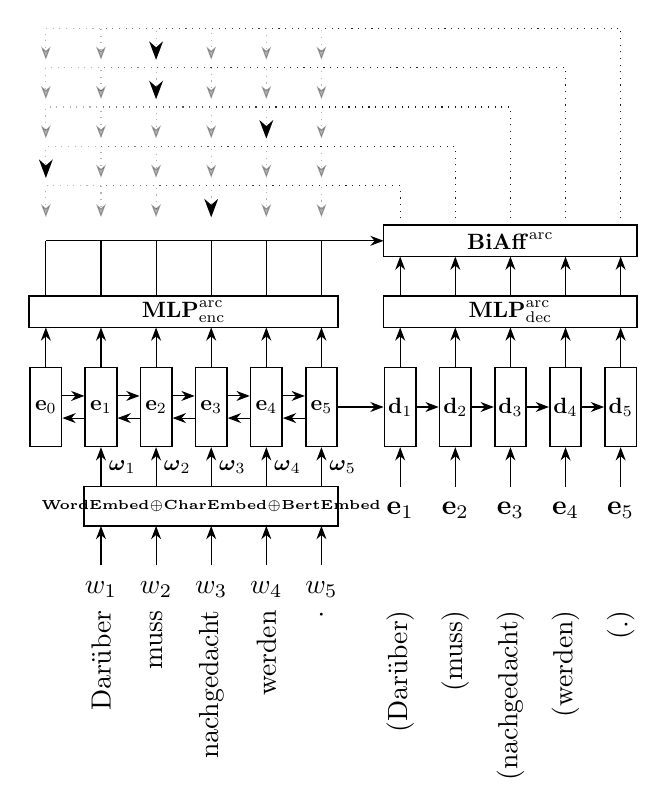
\begin{tikzpicture}[baseline=(current bounding box.north east)]
                \foreach \word / \n / \s in {/0/, Darüber/1/\(w_{1}\), muss/2/\(w_{2}\), nachgedacht/3/\(w_{3}\), werden/4/\(w_{4}\), ./5/\(w_{5}\)}
                {
                    \node[
                        shape=rectangle,
                        inner sep=0pt,
                        fill=none,
                        text=black,
                        anchor=north
                    ] (wd\n) at (0.7 * \n, 0) {\rotatebox{90}{\word}};
                    \node[
                        name=w\n,
                        above=0.2cm of wd\n,
                        text depth=0,
                        text height=1em,
                        inner sep=0
                    ] {\s};
                }
            
                \coordinate[above=0.5cm of w1.north west] (embedbl) {};
                \coordinate[above=1cm of w5.north east] (embedtr) {};
                \draw[semithick] (embedbl) rectangle (embedtr) node [pos=0.5,scale=0.95] {\(\scriptscriptstyle\mathbf{WordEmbed} \oplus \mathbf{CharEmbed} \oplus \mathbf{BertEmbed}\)};
            
                \foreach \n in {0,1,2,3,4,5}
                {
                    \node[
                        above = 0.5cm of {w\n |-embedtr},
                        draw,
                        rectangle,
                        semithick,
                        inner sep=0,
                        minimum width=0.4cm,
                        minimum height=1cm,
                        label={[scale=0.8]center:$\vb{e}_{\n}$}
                    ] (e\n) {};
                }
            
                \foreach \n in {1,2,3,4,5}
                {
                    \draw[-Stealth] (w\n.north) -- (w\n|-embedbl);
                    \draw[-Stealth] (w\n |- embedtr) -- (e\n.south) node[midway, right, scale=0.8] {\(\boldsymbol{\omega}_{\n}\)};
                }
            
                \foreach \n/\m in {0/1,1/2,2/3,3/4,4/5}
                {
                    \draw[-Stealth] ($(e\n.east) + (0, 4pt)$) -- ($(e\m.west) + (0, 4pt)$) {};
                    \draw[Stealth-] ($(e\n.east) - (0, 4pt)$) -- ($(e\m.west) - (0, 4pt)$) {};
                }
            
                \foreach \n/\j in {0/1,1/2,2/3,3/4,4/5}{
                    \node[
                        draw,
                        rectangle,
                        semithick,
                        inner sep=0,
                        minimum width=0.4cm,
                        minimum height=1cm,
                        label={[scale=0.8]center:$\vb{d}_{\j}$}
                    ] (d\j) at ($(e5) + (1 + 0.7 * \n, 0)$) {};
                }
            
                \draw[-Stealth] (e5) -- (d1);
            
                \foreach \n/\m in {1/2,2/3,3/4,4/5}
                {
                    \draw[-Stealth] (d\n) -- (d\m) {};
                }
                \foreach \word/\j in {Darüber/1,muss/2,nachgedacht/3,werden/4,./5}
                {
                    \node[
                        anchor=north,
                        text depth=0,
                        text height=1em,
                        inner sep=0
                    ] (ecopy\j) at (d\j |- embedtr.north) {$\vb{e}_{\j}$} edge[-Stealth] (d\j);
                    \node[
                        shape=rectangle,
                        inner sep=0pt,
                        fill=none,
                        text=black,
                        anchor=north
                    ] at (wd\j.north -| ecopy\j) {\rotatebox{90}{(\word)}};
                }
            
                \coordinate[above=0.5cm of e0.north west] (mlpencbl) {};
                \coordinate[above=0.9cm of e5.north east] (mlpenctr) {};
                \draw[semithick] (mlpencbl) rectangle (mlpenctr) node [pos=0.5,scale=0.8] {\(\mathbf{MLP}_{\text{enc}}^{\text{arc}}\)};
            
                \coordinate[above=0.5cm of d1.north west] (mlpdecbl) {};
                \coordinate[above=0.9cm of d5.north east] (mlpdectr) {};
                \draw[semithick] (mlpdecbl) rectangle (mlpdectr) node [pos=0.5,scale=0.8] {\(\mathbf{MLP}_{\text{dec}}^{\text{arc}}\)};
            
                \foreach \i in {0,1,2,3,4,5}
                {
                    \draw[-Stealth] (e\i.north) -- (e\i |- mlpencbl);
                }
            
                \coordinate[above=0.5cm of {mlpdecbl |- mlpdectr}] (biafbl) {};
                \coordinate[above=0.4cm of {biafbl -| mlpdectr}] (biaftr) {};
                \draw[semithick] (biafbl) rectangle (biaftr) node [pos=0.5,scale=0.8] (biaf) {\(\mathbf{BiAff}^{\text{arc}}\)};
                \foreach \i in {0,1,2,3,4,5}
                {
                    \draw (e\i.north |- mlpenctr) -- (e\i |- biaf);
                }
                \draw[-Stealth] (e0.north |- biaf) -- (biaf.west -| biafbl);
            
                \foreach \j in {1,2,3,4,5}
                {
                    \draw[-Stealth] (d\j.north) -- (d\j |- mlpdecbl);
                    \draw[-Stealth] (d\j |- mlpdectr) -- (d\j |- biafbl);
                    \coordinate (p\j) at ($(biaftr) + (0, 0.5cm * \j)$);
                    \coordinate (q\j) at ($(biaftr) + (0, 0.5cm * \j) - (0, 0.4cm)$);
                }
                \foreach \j in {1,2,3,4,5}
                {
                    \foreach \i in {0,1,2,3,4,5} {
                        \draw[opacity=0.3, dotted,arrows=-Stealth] (biaftr -| d\j) -- (p\j -| d\j) -- (p\j -| e\i) -- (q\j -| e\i);
                    }
                }
                \foreach \j\i in {1/3,2/0,3/4,4/2,5/2}
                {
                    \path[tips,black,thick,dotted,arrows={-Stealth}] (p\j -| e\i) -- (q\j -| e\i);
                }
            \end{tikzpicture}}
        \end{column}
    \end{columns}
    Fixing child \(w_{j}\), the vector \(\mathbf{softmax}(s^{\text{arc}}_{:, j})\) can be interpreted as an estimated probability distribution over potential parents:
            \[
                \hat{p}^{\text{arc}}(w_{i} \mid y_{<j}, w) = \mathbf{softmax}(s_{:,j}^{\text{arc}})_{i}.
            \]
\end{frame}

\subsection{Classification}
\begin{frame}
    \frametitle{Part-of-speech and morphology: quadratic classifier}
    \framesubtitle{Drawing on \textcite{dozat2016deep}.}
    \begin{columns}[t,onlytextwidth]
        \begin{column}[t]{0.52\textwidth}
            \begin{itemize}
            \item Encoder and decoder are shared across tasks. The remaining network is separately trained.
            \item Classification via a bi-affine architecture allows modelling of class probabilities conditional on arcs.
            \end{itemize}

            \textbf{Example:} part-of-speech classification.
            \[
                \vb{e}^{\text{pos}} = \mathbf{MLP}_{\text{enc}}^{\text{pos}}(\vb{e}); \quad \vb{d}^{\text{pos}} = \mathbf{MLP}_{\text{dec}}^{\text{pos}}(\vb{d}).
            \]
        \end{column}
        \begin{column}[t]{0.48\textwidth}
            \raggedleft\scalebox{0.67}{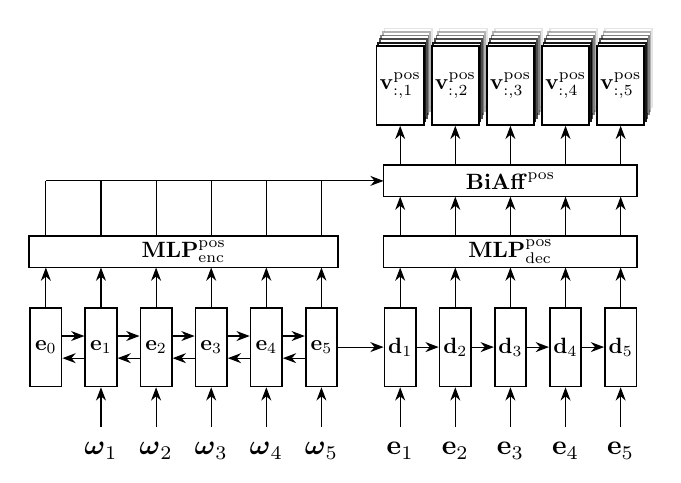
\begin{tikzpicture}[baseline=(current bounding box.north east)]
                \foreach \word / \n in {\texttt{root}/0, Darüber/1, muss/2, nachgedacht/3, werden/4, ./5}
                {
                    \node[overlay,transparent,
                        shape=rectangle,
                        inner sep=0pt,
                        fill=none,
                        text=black,
                        anchor=north
                    ] (wd\n) at (0.7 * \n, 0) {\rotatebox{-90}{\word}};
                    \node[overlay,transparent,
                        name=w\n,
                        above=0.2cm of wd\n,
                        text depth=0,
                        text height=1em,
                        inner sep=0
                    ] {$w_{\n}$};
                }
        
                \coordinate[above=0.5cm of w0.north west] (embedbl) {};
                \coordinate[above=1cm of w5.north east] (embedtr) {};
                \draw[overlay,transparent,semithick] (embedbl) rectangle (embedtr) node [pos=0.5,scale=0.8] {\(\mathbf{WordEmbed} \oplus \mathbf{CharEmbed} \oplus \mathbf{BertEmbed}\)};
        
                \foreach \n in {0,1,2,3,4,5}
                {
                    \draw[overlay,transparent,-Stealth] (w\n.north) -- (w\n|-embedbl);
                    \node[
                        above = 0.5cm of {w\n |-embedtr},
                        draw,
                        rectangle,
                        semithick,
                        inner sep=0,
                        minimum width=0.4cm,
                        minimum height=1cm,
                        label={[scale=0.8]center:$\vb{e}_{\n}$}
                    ] (e\n) {};
                    \draw[overlay,transparent,-Stealth] (w\n |- embedtr) -- (e\n.south);
                }
        
                \foreach \n/\m in {0/1,1/2,2/3,3/4,4/5}
                {
                    \draw[-Stealth] ($(e\n.east) + (0, 4pt)$) -- ($(e\m.west) + (0, 4pt)$) {};
                    \draw[Stealth-] ($(e\n.east) - (0, 4pt)$) -- ($(e\m.west) - (0, 4pt)$) {};
                }
        
                \foreach \n/\j in {0/1,1/2,2/3,3/4,4/5}{
                    \node[
                        draw,
                        rectangle,
                        semithick,
                        inner sep=0,
                        minimum width=0.4cm,
                        minimum height=1cm,
                        label={[scale=0.8]center:$\vb{d}_{\j}$}
                    ] (d\j) at ($(e5) + (1 + 0.7 * \n, 0)$) {};
                }
        
                \draw[-Stealth] (e5) -- (d1);
        
                \foreach \n/\m in {1/2,2/3,3/4,4/5}
                {
                    \draw[-Stealth] (d\n) -- (d\m) {};
                }
                \foreach \word/\j in {Darüber/1,muss/2,nachgedacht/3,werden/4,./5}
                {
                    \node[
                        anchor=north,
                        text depth=0,
                        text height=1em,
                        inner sep=0
                    ] (ecopy\j) at (d\j |- embedtr.north) {$\vb{e}_{\j}$} edge[-Stealth] (d\j);
                    \node[overlay,transparent,
                        shape=rectangle,
                        inner sep=0pt,
                        fill=none,
                        text=black,
                        anchor=north
                    ] at (wd\j.north -| ecopy\j) {\rotatebox{-90}{(\word)}};
                }
        
                \foreach \i in {1,2,3,4,5}
                {
                    \node[
                        anchor=north,
                        text depth=0,
                        text height=1em,
                        inner sep=0
                    ] (omega\i) at (e\i |- embedtr.north) {$\boldsymbol{\omega}_{\i}$} edge[-Stealth] (e\i);
                }
        
                \coordinate[above=0.5cm of e0.north west] (mlpencbl) {};
                \coordinate[above=0.9cm of e5.north east] (mlpenctr) {};
                \draw[semithick] (mlpencbl) rectangle (mlpenctr) node [pos=0.5,scale=0.8] {\(\mathbf{MLP}_{\text{enc}}^{\text{pos}}\)};
        
                \coordinate[above=0.5cm of d1.north west] (mlpdecbl) {};
                \coordinate[above=0.9cm of d5.north east] (mlpdectr) {};
                \draw[semithick] (mlpdecbl) rectangle (mlpdectr) node [pos=0.5,scale=0.8] {\(\mathbf{MLP}_{\text{dec}}^{\text{pos}}\)};
        
                \foreach \i in {0,1,2,3,4,5}
                {
                    \draw[-Stealth] (e\i.north) -- (e\i |- mlpencbl);
                }
        
                \coordinate[above=0.5cm of {mlpdecbl |- mlpdectr}] (biafbl) {};
                \coordinate[above=0.4cm of {biafbl -| mlpdectr}] (biaftr) {};
                \draw[semithick] (biafbl) rectangle (biaftr) node [pos=0.5,scale=0.8] (biaf) {\(\mathbf{BiAff}^{\text{pos}}\)};
                \foreach \i in {0,1,2,3,4,5}
                {
                    \draw (e\i.north |- mlpenctr) -- (e\i |- biaf);
                }
                \draw[-Stealth] (e0.north |- biaf) -- (biaf.west -| biafbl);
        
                \foreach \j in {1,2,3,4,5}
                {
                    \draw[-Stealth] (d\j.north) -- (d\j |- mlpdecbl);
                    \draw[-Stealth] (d\j |- mlpdectr) -- (d\j |- biafbl);
                }
        
                \foreach \j in {1,2,3,4,5}
                {
                    \coordinate (start\j) at (d\j |- {$(biaftr) + (0, 0.5cm)$});
                    \foreach \k/\o in {5/0.1,4/0.3,3/0.5,2/0.7,1/0.9}
                        {
                            \node[
                                draw,
                                draw opacity=\o,
                                rectangle,
                                semithick,
                                inner sep=0,
                                minimum width=0.6cm,
                                minimum height=1cm,
                                anchor=south,
                                fill=white
                            ] (hello) at ($(start\j) + (0.02 * \k, 0.045 * \k)$) {};
                        }
                    \node[
                        draw,
                        anchor=south,
                        rectangle,
                        semithick,
                        inner sep=0,
                        minimum width=0.6cm,
                        minimum height=1cm,
                        fill=white,
                        label={[scale=0.8]center:$\vb{v}^{\text{pos}}_{:,\j}$},
                    ] (posclass\j) at (start\j) {} edge[Stealth-] (d\j |- biaftr);
                }
            \end{tikzpicture}}
        \end{column}
    \end{columns}
    \begin{itemize}
        \item Obtain class \textit{logits} \(\vb{v}^{\text{pos}}\):
            \begin{alignat*}{3}
                \vb{v}^{\text{pos}}_{i,j} &= \mathbf{BiAff}^{\text{pos}}(\vb{e}^{\text{pos}}_{i}, \vb{d}^{\text{pos}}_{j}) \\
                &\coloneqq {\vb{e}^{\text{pos}}_{i}}\tran \mathbf{U}_{\text{h-d}}^{\text{pos}} \vb{d}_{j}^{\text{pos}} +
                        {\vb{e}_{i}^{\text{pos}}}\tran \mathbf{U}_{\text{h-h}}^{\text{pos}} \vb{e}_{i}^{\text{pos}} + U_{\text{h}}^{\text{pos}} \vb{e}_{i}^{\text{pos}} \\
                    &\phantom{\coloneqq}\ + {\vb{d}_{j}^{\text{pos}}}\tran \mathbf{U}_{\text{d-d}}^{\text{pos}} \vb{d}_{j}^{\text{pos}} + U_{\text{d}}^{\text{pos}} \vb{d}_{j}^{\text{pos}} + \vb{u}_{\text{bias}}^{\text{pos}}.
            \end{alignat*}
    \end{itemize}

    Fixing child \(w_{j}\), the vector \(\mathbf{softmax}(\vb{v}_{i,j}^{\text{pos}})\) can be interpreted as an estimated probability distribution over its parts-of-speech conditional on having an arc to \(w_{i}\):
            \[
                \hat{p}^{\text{pos}}(c \mid w_{i}, y_{<j}, w) = \mathbf{softmax}(\vb{v}^{\text{pos}}_{i,j})_{c}.
            \]
\end{frame}

\subsection{Inference and Training}
\begin{frame}
    \frametitle{Inference and Training}
    \setlength{\abovedisplayskip}{0pt}
\setlength{\belowdisplayskip}{0pt}
\setlength{\abovedisplayshortskip}{0pt}
\setlength{\belowdisplayshortskip}{0pt}
    \begin{block}{Inference}
        Given \(w=\qty(w_{i})_{i=1}^{L}\), estimate \(y = \qty(y_{i})_{i=1}^{L}\) via \textit{maximum likelihood}:
        \begin{align*}
            \hat{y} &= \mathop{\underset{y}{\operatorname{arg\,max}}} \Bigg\{  \prod_{i=1}^{L} \Big\{ \hat{p}_{w}(y_{i}^{\text{arc}} \mid y_{<i}) \hat{p}_{w}(y_{i}^{\text{lab}} \mid y_{i}^{\text{arc}}, y_{<i}) \\[-2.5em]
            &\phantom{\ = \mathop{\underset{y}{\operatorname{arg\,max}}} \Bigg\{ \prod_{i=1}^{L} \Big\{} \cdot \hat{p}_{w}(y_{i}^{\text{ord}} \mid y_{i}^{\text{arc}}, y_{<i}) \hat{p}_{w}(y_{i}^{\text{pos}} \mid y_{i}^{\text{arc}}, y_{<i}) \hat{p}_{w}(y_{i}^{\text{morph}} \mid y_{i}^{\text{arc}}, y_{<i}) \Big\} \Bigg\}.
        \end{align*}
    \end{block}

    The feasible region is very large, so the maximisation is approximated via \textit{beam search}.

    \begin{block}{Training}
        Minimise the \textit{cross-entropy} between \(\hat{p}\) and the empirical distribution present in the dataset \((w^{n}, y^{n})_{n=1}^{N}\):
        
        \begin{align*}
            \mathop{\underset{\hat{p}}{\min}} \Bigg\{ - \sum_{n=1}^{N} \log \prod_{i=1}^{L_{n}} \Big\{ & \hat{p}_{w}({y_{i}^{n}}^{\text{arc}} \mid y_{<i}^{n}) \hat{p}_{w}({y_{i}^{n}}^{\text{lab}} \mid {y_{i}^{n}}^{\text{arc}}, y_{<i}^{n}) \\[-2.25em]
            & \cdot \hat{p}_{w}({y_{i}^{n}}^{\text{ord}} \mid {y_{i}^{n}}^{\text{arc}}, y_{<i}^{n}) \hat{p}_{w}({y_{i}^{n}}^{\text{pos}} \mid {y_{i}^{n}}^{\text{arc}}, y_{<i}^{n}) \hat{p}_{w}({y_{i}^{n}}^{\text{morph}} \mid {y_{i}^{n}}^{\text{arc}}, y_{<i}^{n}) \Big\} \Bigg\} \\
            &= \mathop{\underset{ \hat{p}}{\min}} \qty{\text{loss}^{\text{arc}} + \text{loss}^{\text{lab}} + \text{loss}^{\text{ord}} + \text{loss}^{\text{pos}} + \text{loss}^{\text{morph}}}.
        \end{align*}
    \end{block}

    This is approximated via \textit{SGD} with \textit{Nesterov momentum}.
\end{frame}

\section{Data and Results}
\begin{frame}
    \frametitle{Performance metrics}
    The TIGER treebank is a widely-used corpus of \(\sim\!50\,000\) constituency trees. Its main textual basis is the \textit{Frankfurter Rundschau}.
    \begin{itemize}
        \item \(97\,\%\) of the dataset is usable as training examples, with train/dev/test split of \(80/10/10\,\%\).
    \end{itemize}

    \begin{columns}[onlytextwidth]
        \begin{column}[t]{0.48\textwidth}
            \begin{table}
                \begin{tabular}[t]{@{}
                    >{\arraybackslash}p{(\textwidth - 6.5em)}@{}
                    >{\centering\arraybackslash}p{3em}@{}
                    >{\centering\arraybackslash}p{4em}@{}}
                    \toprule
                    \textbf{Model} & \textbf{F1} & \textbf{Disc. F1} \\ \midrule
                    \textls[-70]{F.-González \& G.-Rodríguez (\citeyear{fernandez2022multitask2})} & 89.8 & 71.0 \\
                    Corro (\citeyear{corro2020span}) & \textbf{90.0} & 62.1 \\
                    Chen \& Komachi (\citeyear{chen2023discontinuous}) & 89.6 & 70.9 \\
                    \midrule
                    \textbf{This work} & 89.5 & \textbf{82.2} \\ \bottomrule
                \end{tabular}

                \caption{Comparison of overall F1-score (\%) and F1-score measured only on discontinuous constituents (disc. F1). Calculated using \texttt{disco-dop} \parencite{van2016data} as standard practice. All models configured with BERT.}
            \end{table}
        \end{column}
        \begin{column}[t]{0.48\textwidth}
            \begin{table}
                \begin{tabular}[t]{@{}
                    >{\arraybackslash}p{(\textwidth - 7.25em)}@{}
                    >{\centering\arraybackslash}p{2.3em}@{}
                    >{\centering\arraybackslash}p{5em}@{}}
                    \toprule
                    \textbf{Model} & \textbf{\texttt{pos}} & \textbf{\texttt{morph}} (avr) \\ \midrule
                    \textcite{kondratyuk2018lemmatag} & 98.58 & 98.97 \\
                    \textcite{muller2013efficient} & 98.20 & 98.27 \\
                    \textls[-20]{Schnabel \& Schütze (\citeyear{schnabel2014flors})} & 97.50 & 97.76 \\
                    \midrule
                    \textbf{This work} & \textbf{99.16} & \textbf{99.54} \\ \bottomrule
                \end{tabular}

                \caption{Comparison of part-of-speech (\texttt{pos}) and morphology accuracies (\%). Morphology accuracies are the average of accuracies for \texttt{case}, \texttt{degree}, \texttt{gender}, \texttt{mood}, \texttt{number}, \texttt{person} and \texttt{tense}.}
            \end{table}
        \end{column}
    \end{columns}
\end{frame}
\section{Appendix}

\nocite{gleim2019practitioner}
\nocite{eger2016lemmatization}


\begin{frame}[allowframebreaks]
    \frametitle{Bibliography}
    \printbibliography
\end{frame}

\appendix

\section{Mathematical justification of bi-affine classifier}
\begin{frame}
    \frametitle{Appendix: Mathematical justification of bi-affine classifier}
    Notation has been simplified for presentational clarity. Take a single class \(c\) and suppose
    \[
        \mqty[\vb{e}_{i} \\ \vb{d}_{j}] \, \Big| \, c \sim \mathcal{N}\qty(\mqty[\boldsymbol{\mu}_{c} \\ \boldsymbol{\phi}_{c}], \mqty[\mathbf{A}_{c} & \mathbf{Q}_{c} \tran \\ \mathbf{Q}_{c} & \mathbf{B}_{c}]^{-1}).
    \]

    The conditional log-likelihood of \(c\) is the following affine quadratic form:
    {\begin{align*}
        v_{i,j}^{c} &= \log p(\vb{e}_{i} \mid c, \vb{d}_{j}) = k^{c} -\frac{1}{2} ((\vb{e}_{i} - \boldsymbol{\mu}_{c}) - \mathbf{A}_{c}^{-1} \mathbf{Q}_{c}\tran(\vb{d}_{j} - \boldsymbol{\phi}))\tran \mathbf{A}_{c} (\vb{e}_{i} - \boldsymbol{\mu}_{c}) - \mathbf{A}_{c}^{-1} \mathbf{Q}_{c}\tran(\vb{d}_{j} - \boldsymbol{\phi}) \\
        &= \tikzmarknode{h-d-source}{\vb{e}_{i}\tran \mathbf{Q}_{c} \tran\vb{d}_{j}}
            - \tikzmarknode{h-h-source}{\frac{1}{2} \vb{e}_{i}\tran \mathbf{A}_{c}\vb{e}_{i}}
            - \tikzmarknode{d-d-source}{\frac{1}{2} \vb{d}_{j}\tran \mathbf{Q}_{c} \mathbf{A}_{c}^{-1} \mathbf{Q}_{c}\tran \vb{d}_{j}}
            + \tikzmarknode{h-source}{\qty(\boldsymbol{\mu}\tran \mathbf{A}_{c} - \boldsymbol{\phi}\tran \mathbf{Q}_{c})\vb{e}_{i}} + \tikzmarknode{d-source}{(\boldsymbol{\phi}\tran \mathbf{Q}_{c} \mathbf{A}_{c}^{-1} \mathbf{Q}_{c}\tran - \boldsymbol{\mu}\tran \mathbf{Q}\tran)\vb{d}_{j}} \\
             & \qquad \qquad \qquad \qquad \qquad \qquad \qquad \qquad \qquad \qquad \qquad \qquad  \mathrel{\tikzmarknode{before-bias-source}{+}} \tikzmarknode{bias-source}{\boldsymbol{\mu}\tran\mathbf{Q}_{c}\tran\boldsymbol{\phi}
            -  \frac{1}{2} \boldsymbol{\phi}\tran\mathbf{Q}_{c}\mathbf{A}_{c}^{-1}\mathbf{Q}\tran \boldsymbol{\phi} + k_{c}} \\
        &= c\text{th row of }
        \tikzmarknode{h-d-dest}{\vb{e}_{i}\tran \mathbf{U}_{\text{h-d}} \vb{d}_{j}}
           + \tikzmarknode{h-h-dest}{\vb{e}_{i}\tran \mathbf{U}_{\text{h-h} }\vb{e}_{i}}
           + \tikzmarknode{d-d-dest}{\vb{d}_{j}\tran \mathbf{U}_{\text{d-d}} \vb{d}_{j}}
           + \tikzmarknode{h-dest}{U_{\text{h}} \vb{e}_{i}}
           + \tikzmarknode{d-dest}{U_{\text{d}} \vb{d}_{j}}
           + \tikzmarknode{bias-dest}{\vb{u}_{\text{bias}}}
    \end{align*}
    }%

    \begin{tikzpicture}[remember picture, overlay]
        \foreach \n in {h-d,h-h,d-d,h,bias}
        {
            \node [draw, fill=green, opacity=0.2, fit=(\n-source), inner sep=1pt] (highlight\n) {};
            \draw[-Stealth] (highlight\n)  -- (\n-dest);
        }

        \node [draw, fill=green, opacity=0.2, fit=(d-source), inner sep=1pt] (highlightd) {};        

        \coordinate (c11) at (highlighth.south east);
        \coordinate (c12) at (highlighth.south east |- highlightbias.north west);
        \coordinate (c1) at (barycentric cs:c11=5,c12=1);

        \coordinate (c21) at (highlightbias.west);
        \coordinate (c22) at (highlightbias.north west |- highlighth.south east);
        \coordinate (c2) at (barycentric cs:c21=1,c22=2);

        \draw[-Stealth] plot [smooth, tension=0.7] coordinates { (highlightd.south west) (c1) (c2 -| before-bias-source) ($(before-bias-source.west) - (0.5ex, 0)$) (d-dest.north)};
    \end{tikzpicture}

    \textbf{Memory-efficient implementation:} under conditional normality, the affine quadratic transformation can be computed as
    \[
        v_{i,j}^{c} = k^{c} + \norm{W_{h}^{c} \vb{e}_{i} + W_{d}^{c}\vb{d}_{j} + \vb{w}^{c}}_{2}
    \]
\end{frame}
\end{document}